\section{Evaluation}
\label{sec:eval}

% \begin{itemize}
%   \item Experiment on datas from the Bureau of Transportation Statistic (\url{http://www.transtats.bts.gov/Fields.asp?Table_ID=236}) to evaluate flight delays by airport
%   \item Infrastructure based on ONE cluster, VM 16.04 LTS (GNU/Linux 4.4.0-53-generic x86\_64), Docker 1.13.0-rc3, Docker Swarm 1.2.5 (discovery: Consul v0.5.2)
%   \item Hardware?
% \end{itemize}
This section reports on our evaluation of \SYS.
First, we present our evaluation settings.
Secondly, we detail the real-world dataset used in our experiments.
Finally, we analyze some preliminary benchmarks, namely throughput and scalability.

\textbf{Evaluation settings.}
We deploy a cluster of \emph{virtual machines} (VM) based on Ubuntu 16.04 LTS \rp{This should change to 14.04, due to the compatibility requirement of SGX SDK} and running a daemon Docker (v.1.13.0-rc3).
Each VM is set with 2 CPU cores and 2GB RAM, and interconnected using a switched 1~Gbps network.
Nodes join a Docker Swarm cluster~\cite{docker:swarm_2016} (v1.2.5), using Consul~\cite{consul} (v0.5.2) as discovery service.
Each VM only executes one single Docker instance, to prevent cross-container interferences~\cite{koh2007analysis}.
%A single-one container is launch on each node.
Containers leverage the Docker overlay network to communicate to each other.
\vs{add SGX things}

\textbf{Dataset.} In our experiments, we process a real dataset released by the \emph{American Bureau of Transportation Statistic}~\cite{rita:bts}.
%including each flight's departure and arrivals\cite{statistical_computing:data}.
The dataset reports on the flight departures and arrivals of 20 air carriers~\cite{statistical_computing:data}.
We implement a benchmark application atop of \SYS to compute average delays and the total of delayed flights for each air carrier.
%These datas report flights departures and arrivals\cite{rita:bts} and are available on the Statistical Computing\cite{statistical_computing:data}.
We design and implement the full processing pipeline, that (i) parses the input datasets (in a comma-separated-value format) to data structure (\textsf{map}), (ii) filters data by relevancy (\emph{i.e.}, if the data concerns a delayed flight), and (iii) finally reduces it to compute the wanted informations.\footnote{This experiment is inspired by Kevin Webber's blog entry \emph{Diving into Akka Streams}: \url{https://blog.redelastic.com/diving-into-akka-streams-2770b3aeabb0}.}
We use the 4 last years of the available dataset (from 2005 to 2008), for a total of 28 millions of entries to process and 2.73 GB of data.
\vs{Update with the details of other datasets if any}

\textbf{Micro-Benchmark: Lua in SGX.}
\vs{NEW: here we show the overhead of executing Lua code inside/outside SGX enclaves. We should use well-known Lua benchmarks (maybe there are few in Lua's own test suite or come up with something that shows the trade-offs.)}
\vs{we should explore a bit the design space: how much data should be sent at once into the enclave before side-effects kick-in ? upon these results, we choose the proper parameter for the follow-up experiments.}

To estimate the cost of enclaved function calls we averaged the time it took to do one milion calls with no data transfers. 
While normal function calls took 23.6 $ns$, enclaved calls took on average 2.35 $\mu s$, i.e., two orders of magnitude worse. 
We then assessed the cost of copying data from the unshielded execution to the enclave and compared with the time it took to natively do the same. 
We initialized a buffer of 100 MB with random data and copied its content by chunks of increasing sizes, with one function call per chunk. 
Figure~\ref{fig:sgxmemcpy} shows the results. When using smaller chunks, the function call overhead plays an important role in the total time, which steadly drops until we send chunks of 64 KB. Then we can notice an abrupt growth for the enclaved execution time, which can probably be credited to cache phenomena \rp{???}.

\begin{figure}[t!]
  \centering
  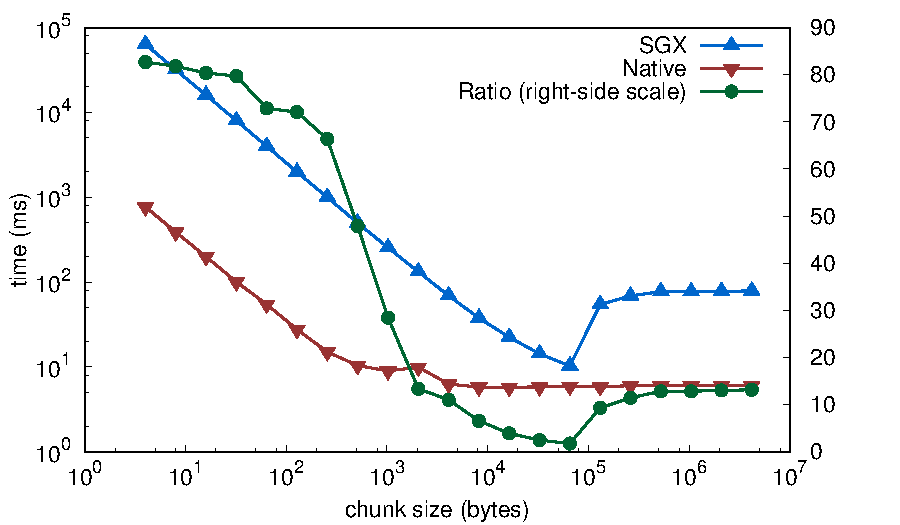
\includegraphics[scale=0.45]{plots/memcpy.pdf}
  \caption{Time to copy 100 MB of memory}
  \label{fig:sgxmemcpy}
\end{figure}

Planned benchmarks:
\begin{itemize}
	\item overhead of the Lua benchmarks from \url{https://github.com/ltratt/vms_experiment/tree/master/benchmarks}
\end{itemize}
\textbf{Benchmark: throughput.}
This benchmark shows the upload throughput observed across the whole cluster while streaming the dataset as fast as possible from the source nodes into the processing pipeline.
We gather bandwidth measurements by exploiting Docker's own monitoring and statistical module.
%Throughput accross containers wrapping each node of the processing pipeline are measured from Docker stats.
The statistics are gathered at runtime while the experiment is executing.
%During the experiment, we retrieve all the data stats for each container.
%In particular, \texttt{txbytes} stats are extracted to measure containers output throughput.
We report on our results in Figure~\ref{fig:throughput}.
In this scenario, 4 nodes concurrently inject the input dataset into the processing pipeline, each one using a subset of the full dataset.
However, only one worker process is used for each step of the processing pipeline.
We use a representation based on stacked percentiles.
The white bar at the bottom represents the minimum value, the pale grey on top the maximal value.
Intermediate shades of grey represent the 25th, 50th–, median–, and 75th percentiles.
For instance, the median throughput at 200\,seconds into the experiment almost hits 2,500\,kB/s, meaning that 50\,\% of the nodes in that moment are outputting data at 2,500\,kB/s or less.
%These datas are computed to be plotted together by percentile, as shown on figure \ref{fig:throughput}.\ah{maybe it could be relevant to put three plots, corresponding to experiments 4-datas-1-worker, 4-datas-2-workers and 4-datas-4-workers}
With the current implementation, we observe a peak of 10\,MB/s upload throughput into the processing stages.%\vs{for the future, it'd be interesting to know which stage is the fastest one}
%\ah{I gonna measure throuput between two containers run on a swarm cluster, using iperf, for comparison purpose}


\begin{figure}[t!]
  \centering
  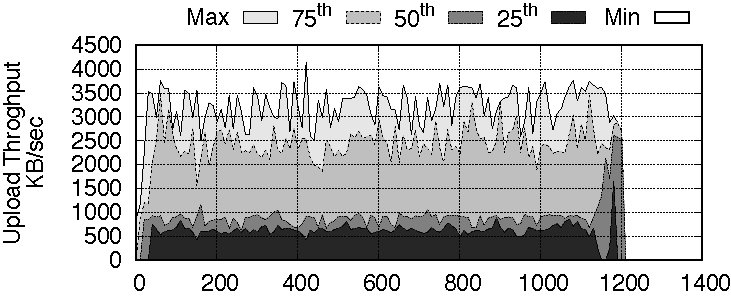
\includegraphics[scale=0.7]{images/tput_upload_4-datas-1-worker.pdf}
  \caption{Upload Throughput, single source. The middleware framework completes the processing of the dataset in 1,200\,seconds, with a peak of 4\,MB/s and an overall average throughput of 2.3\,MB/s}
  \label{fig:throughput}
\end{figure}

\vs{We should then extend this section to present how the TPUT is affected by having few/all streams going through the enclaves. This would be an interesting/useful plot as it provides useful insights.}

\textbf{Benchmark: scalability.} We conclude this preliminary by presenting scalability results of the \SYS framework.
In particular, we scale up each stage of the processing pipeline, up to 4\,workers per stage.
For each of the configurations, the experiment is repeated 20\,times.
We show average and standard deviation of the overall completion time to process the full dataset.
Figure~\ref{fig:scalability} depicts these results.
%Scalability of \SYS is evaluated by processing these datas 20 times on 3 different pipeline topology: using 1, 2 or 4 workers for each step of the pipeline.
We observe that by doubling the number of workers from the initial configuration achieves a 2$\times$ speed-up of the overall processing time, that is from 20\,minutes to less than 10\,minutes.
Conversely, we do not observe similar improvements when using 4\,workers.
%Results are represented on figure \ref{fig:scalability}, and show clearly better performances between the experiment using only one worker by task, and the one using 2 workers.
%In an other hand, using 4 workers instead of 2 does not show any performance improvement.

\begin{figure}[t!]
  \centering
  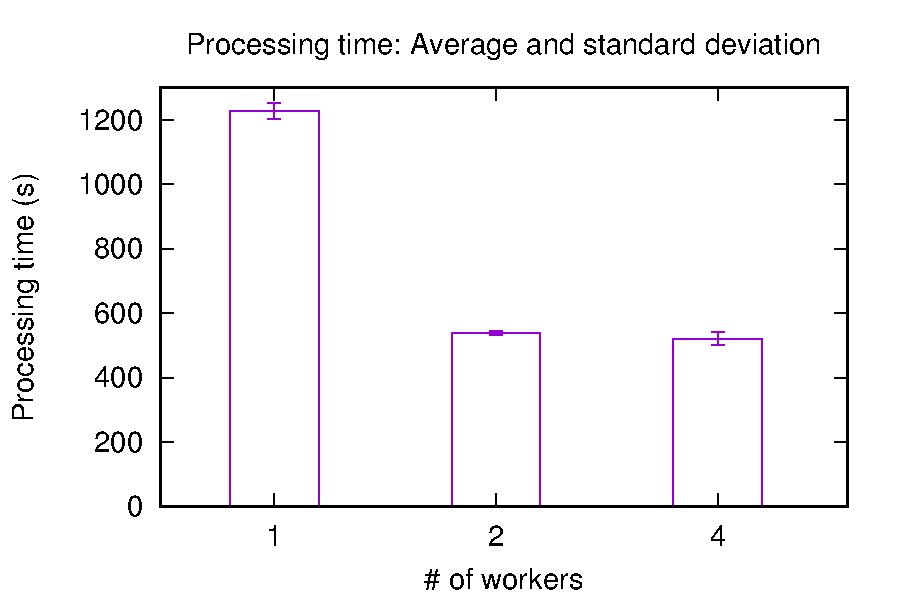
\includegraphics[scale=0.5]{images/avg_stdev_4_streams}
  \caption{Scalability: processing time, average and standard deviation. The experiment is repeated 20 times.\vs{plot can be improved, check if we actually keep this}}
  \label{fig:scalability}
\end{figure}

We believe this behavior can be explained by existing bottlenecks in the pipelining infrastructure, lack of optimization in the application logic as well as tuning options of the \zmq queues.
These hypotheses are confirmed by observing the throughput of the system once we increase the processing workers to 2 and 4 in Figure~\ref{fig:throughput2} and Figure~\ref{fig:throughput4}, respectively.
We observe the following facts.
First, the system is far from saturating the network's available bandwidth, hitting a peak of 10\,MB/s.
Second, a small percentage of nodes consumes much more bandwidth than the other components.
We intend to further investigate these effects as part of our future work, as we are going to elaborate in the following section.

\begin{figure}[t!]
  \centering
  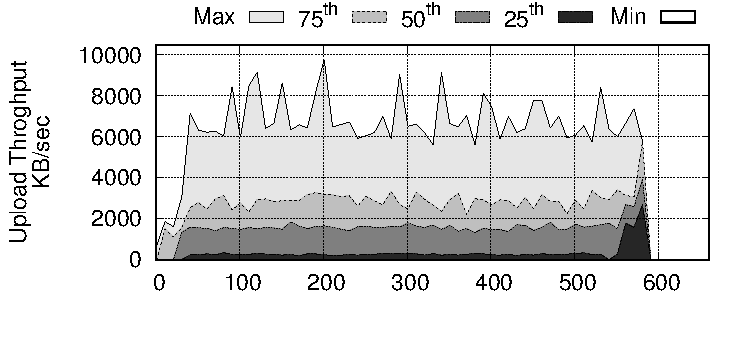
\includegraphics[scale=0.7]{images/tput_upload_4-datas-2-workers.pdf}
  \caption{Upload throughput, 2 concurrent processing workers by pipeline stage. Peak throughput at 10MB/s.}
  \label{fig:throughput2}
  \vspace{0.5cm}
  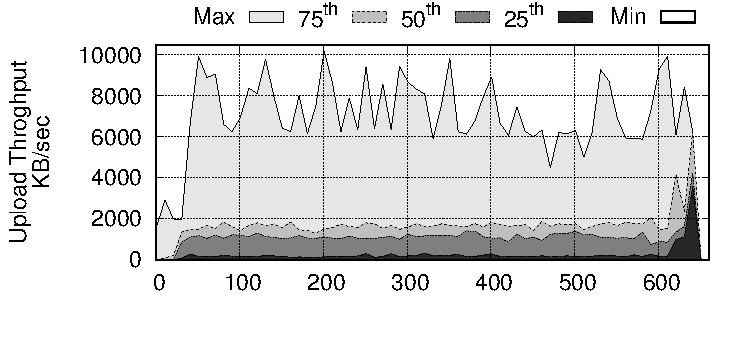
\includegraphics[scale=0.7]{images/tput_upload_4-datas-4-workers.pdf}
  \caption{Upload throughput, 4 concurrent processing workers by pipeline stage. Peak throughput at 10MB/s.}
  \label{fig:throughput4}
\end{figure}

%The latter observation can be explained by the fact that each job in our experiment is very simple and executed too quickly by the workers, compared to the throughput capacity of the communication between two steps of the process pipeline.
%This may be due to the limitation of the network bandwith capacity, when the cost of data communication accross nodes is higher than the one of data computation, as described by the Gunther's Universal Law of Computational Scalability\cite{gunther1993simple}, where the relative capacity of a computational platform is inversely proportional to the sum of the levels of contention (e.g., queueing for shared resources) and coherency delay (i.e., latency for data to become consistent) in the system.
%In an other hand, it may also be due to the limitation of the router bandwith, the improvement of which is a part of our future work.
